
% \usepackage{graphicx}
% \usepackage{palatino}
% \usepackage{url}
% \usepackage{hyperref}

% %\usepackage{a4-mancs}

% \usepackage{handout}

% \begin{document}

\chapter{Report writing and Digital Typography}
\begin{refsection}
  
  \minitoc

  \notesurl{latex-exercise}

\section{Introduction}

\LaTeX\ is a document preparation system that is fundamentally
different to anything that you are likely to have seen before. It's
used worldwide by publishers, academics and scientists.

\LaTeX\ was written by Leslie Lamport, an American computer scientist now working at Microsoft Research.  It's actually built on top of another system called \TeX, a computer typesetting system designed by one of the world's most influential Computer Scientists, Donald Knuth of Stanford University. Knuth has said that he designed \TeX\ for ``the creation of beautiful books---and especially for books that contain a lot of mathematics.'' \citep{knuth1984}. Figure \ref{figure:knuthlamport} shows what these eminent men look like.

  
So what's the purpose of \LaTeX ? It's purely a layer of software to make \TeX\ easier to use in everyday situations. This is a good idea, because although \TeX\ is amazingly powerful, it operates at a very low-level, which makes it hard for non-expert users.

\begin{figure}[hb]
  \centering
     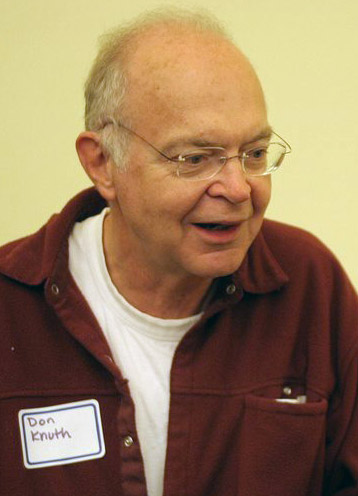
\includegraphics[height=6cm]{images/knuth.png}
\quad\quad  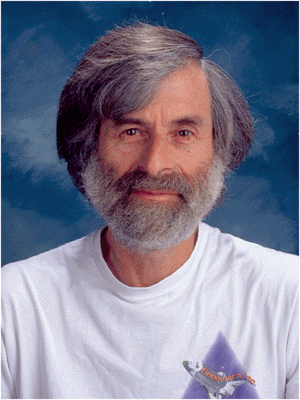
\includegraphics[height=6cm]{images/lamport.png}
\caption{Don Knuth and Leslie Lamport.}\label{figure:knuthlamport}
\end{figure}

\subsection{Pronunciation}
\label{sec:pronunciation}
  The name \TeX\ is intended by its creator to be pronounced with the final consonant as in the word loch or the name Bach, but English speakers often pronounce it like the first syllable of technical. The first syllable of \LaTeX\ is pronounced as in 'lay'\footnote{The Greek prefix `tex' means `art' as well as `technology', so it's a very nicely chosen name for a piece of software that produces such beautiful output. Knuth explained \citep{knuth1984} that one should ``pronounce the X of TeX as a Greek chi, not as an `x', so that TeX rhymes with the word blecchhh.''. We're not too sure that helps much, unless you are confident in your pronunciation of the word `blecchh'. Maybe it's an American thing.}.


\section{Why \LaTeX?}
\label{sec:why}
 Before we go any further, why do we think \LaTeX\ is important for you---a Computer Science student---to know about? Here are some reasons, in no particular order.

\begin{itemize}
\item \LaTeX\ and \TeX\ are superb examples of Computer Science in action. \TeX\ was designed by Knuth from first principles---in other words, ``from scratch''.  \TeX\ is actually a programming language, and \LaTeX\ is a set of functions defined in the \TeX\ language. The \TeX\ ``compiler''  (the source code is publicly available in C and Pascal)  reads a \TeX\ program and outputs documents. \TeX\ is completely self-contained, designed to be portable to any computer architecture. For example, it implements its own stack and heap (with garbage collection), and it does fixed-precision arithmetic. 
\item \LaTeX\ is a new, interesting, way for you to think about preparing documents. 
\item \LaTeX\ has a practical advantage for the writer, in that it helps you think more about \emph{what} you want to write, rather than worrying about \emph{how it looks}.
\item \LaTeX\ is a powerful tool for professional scientific documentation, and as Computer Scientist, you should know about it.
\item \LaTeX\ files are just `plain text', so can easily be created programatically. For example, some of the slides used for COMP16120 are generated automatically from the source of John's book; both are typeset using \LaTeX. The program \texttt{labprint} also produces its output using \LaTeX, using information drawn from XML configuration files and Arcade.
  
\item Using \LaTeX\ is actually quite satisfying, and the quality of its output may surprise you.
\end{itemize}

In this exercise you are going to write at least two documents using \LaTeX. You should also write brief notes in your logbook about how \LaTeX\ works and what commands you used inside the source of your documents. A portion of the assessment will be based on your logbook. 

Nevertheless, when you have completed as much as you are going to do, you should run \texttt{submit} and (when next in the school) \texttt{labprint}.

\section{Some history: printing mathematics}

Mathematics is hard to print, on paper, and on the Web (many websites resort to GIF or JPG images of maths formulae, which usually look horrible. MathML is a better way, though not yet widely used).

In days before computers, books and newspapers were printed with ``movable type'', made from lots of little blocks of metal each with letters, numbers and symbols standing in relief, which when inked left an impression on the paper (see Figure \ref{figure:movabletype}). The job of the printer (the printer here, of course, being person, not a bit of electronics) was to gather together all the blocks in the right order between two horizontal strips of wood to create a line of the document, and then to assemble all those lines from top to bottom of a page. Thus the term `type setting': an incredible task, when you think about it. In the printer's workshop, by the way, between jobs the blocks of metal were stored in wooden boxes called `cases'. Letters like a, b and c were stored in one case; letters like A, B, and C were stored in a case sitting on top of that. So, a lower case, and an upper case. These terms may ring a bell.

\begin{figure}
\centerline{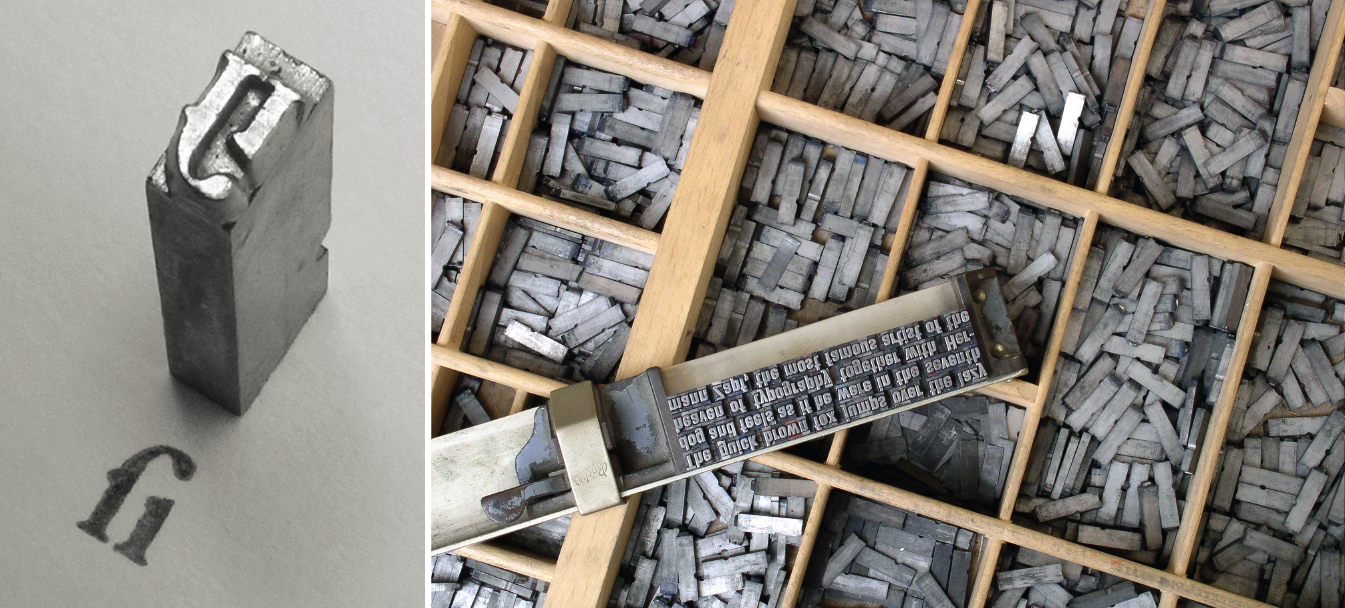
\includegraphics[width=12cm]{images/movable-type.png}}
\caption{On the left, a piece of cast movable type in the Garamond font. On the right, a case of cast metal type pieces and typeset matter in a composing stick. The text reads `The quick brown fox jumps over the lazy dog and feels as if he were in the seventh heaven of typography together with Hermann Zapf, the most famous artist of the' (this document is typeset in a font called Palatino, created by Hermann Zapf. You may have also seen 'Zapf Dingbats' in the font lists of various desktop applications. Now you know why.)} \label{figure:movabletype}
\end{figure}

As technology progressed, machines controlled by typewriters would mechanically juggle the blocks into the right order. This conceptual model, by the way, is the basis on which \TeX\ operates. Only now, the metal blocks are little pieces of data, arranged into data structures. 

The one thing that traditional printers hated was dealing with the typesetting of mathematics, and they would charge extra for do it. It was incredibly fiddly: to get the equations looking right they had to squeeze in extra bits of metal horizontally and vertically. 

When computers entered the printing world, attempts to print mathematics were limited by the printing technology available. It took a long time to reach the point where computers could typeset mathematics beautifully, and that was the outstanding achievement of Knuth's \TeX.

Let's look at a quick example of the quality you get from \LaTeX, with a very simple formula that you'll recognise:

\[ x = \frac{-b \pm \sqrt{b^2-4ac}}{2a} \]
%
We'll revisit how \LaTeX\ typesets mathematics in Section~\ref{mathssection}.

\section{To WYSIWYG or not to WYSIWYG?}
Up until now, you have probably used wordprocessing applications such as Microsoft Word to create essays, letters and other (probably fairly short) documents. You most likely know that the majority of modern word processors use a paradigm called WYSIWYG, or What You See Is What You Get, which means that you can modify the visual style of the document you're working on by selecting the relevant bits, and then choosing different attributes such as font size or colour using a GUI. In many ways this seems like such a sensible and obvious way of doing things, that you might be wondering why it even has a special name. The reason is a historical one: in the early days of computing, long before graphical window managers became the norm, and when all you could display on screen was fixed-width ASCII text in whatever the system's default font was, wordprocessors (e.g. Figure \ref{figure:wordperfect}) only allowed you to format documents by using special sequences of characters to cause particular effects. But these effects were only visible when the document was printed. So if you wanted a word to appear in \textbf{bold text}, in the wordprocessor you might write something like \texttt{[bold]hello world[/bold]}: what you saw on screen was \emph{not} a direct reflection of what appeared on the printed page. If you've written any HTML, however, this process of `marking up' text may be familiar. As computers moved to displays able to draw things other than raw characters on screen, wordprocessors became capable of using multiple fonts and styles, as well as graphics, and a new generation of applications appeared where what you saw on screen \emph{was} an accurate reflection of how it would appear when printed: what you see (on screen), is what you get (on paper). 

\begin{figure}
\centerline{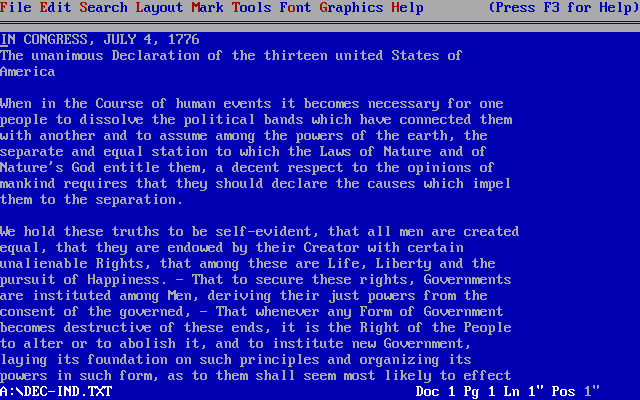
\includegraphics[width=12cm]{images/wordperfect.png}}
\caption{A screenshot of Wordperfect 5.1, running in Microsoft DOS circa 1989.}\label{figure:wordperfect}
\end{figure}

\begin{figure}

\begin{verbatim}
                \documentclass{article}
                \begin{document}
                \textbf{Hello world}
                \end{document}
\end{verbatim}
\center{(a)}
\begin{verbatim}
                <html>
                  <body>
                     <b>Hello world</b>
                  </body>
                </html>
\end{verbatim}
\center{(b)}

\caption{Examples of the words `hello world' in bold text typeset (a) \LaTeX\ and (b) HTML}\label{figure:helloworld}
\end{figure}


The huge advantage of WYSIWYG is that it's really easy to understand what's going on, and most people can create reasonably nicely formatted documents with relatively little effort. For short informal documents, one-off letters, memos and such, WYSIWYG works quite nicely. But if you've ever tried writing anything much longer, or that includes images and tables, you may have already started to see where the paradigm breaks down. For example, if you write ``Figure \ref{figure:menandcheeses} on page \pageref{figure:menandcheeses}  shows a picture of some men looking at cheese'', but then later on edit your document to include some more text at the start, and a new picture of a some broccoli (as in Figure \ref{figure:broccoli}), you'd have to search through your report to find all mentions of `Figure \ref{figure:menandcheeses}' and `page \pageref{figure:menandcheeses}' and manually update them to reflect the new numbering. This might be fine if you have two figures and five pages; but for a hundred-page report containing lots of pictures, you can see how this becomes tedious and error prone very quickly. 

\begin{figure}
\centerline{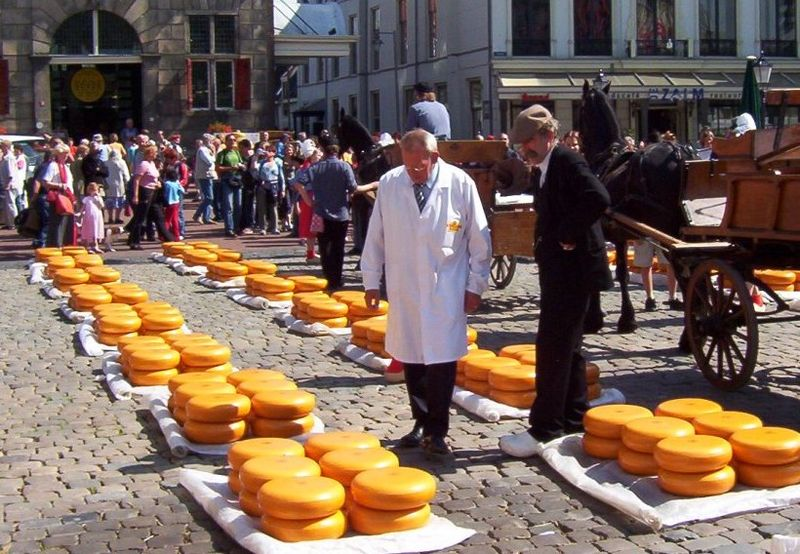
\includegraphics[width=10cm]{images/men-and-cheese.jpg}}
\caption{Some men, possibly Dutch, looking at cheeses.}\label{figure:menandcheeses}
\end{figure}

\begin{figure}
\centerline{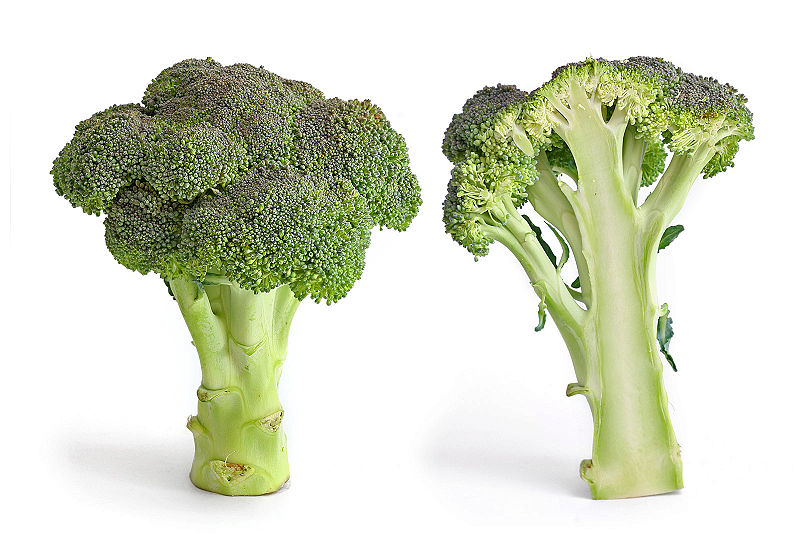
\includegraphics[width=10cm]{images/broccoli.jpg}}
\caption{Some broccoli.}\label{figure:broccoli}
\end{figure}

\section{Style and content}

The other thing about WYSIWYG is that it puts you entirely in control of the visual layout and style of your article, and this isn't necessarily a good thing for two reasons. First, it means that instead of focusing on the content and structure of what you're writing, it makes it easy to get distracted by tinkering with the layout and style. And although layout and style are of course important if you want to create a professional-looking document, they are definitely always secondary to content and structure. Second, it means that you are, well, entirely in control of the visual layout and style of your article. And although it might not be obvious up-front, such control is not necessarily a good thing unless you really know what you're doing (and unless you are a talented graphic designer with a deep understanding of typography, you almost certainly don't\footnote{Don't take this personally; we're in the same boat. If you think that this document is nicely formatted, that's all down to \LaTeX, not us!}). Creating documents that are aesthetically pleasing and easy to read is rather a specialist skill with its origins going all the way back to Caxton's invention of the printing press in the fifteenth century.  Over the years, typographers have honed their skills, arriving at complex rules and heuristics that determine the optimum number of characters on a line, ideal relative and absolute font sizes, spacings, margins, figure placement and so on that lead to attractive---and most importantly---readable documents. You could of course learn all these rules, and make sure you implement them manually using your favourite WYSIWG editor, but that's not what a Computer Science degree is about. The \LaTeX\ system implements many of these rules, making decisions for you about the best way to lay your document out on the page. This allows you to concentrate on creating good quality content, safe in the knowledge that \LaTeX\ will do a good job of laying it out for you. The idea of separating out `content' from `presentation' is something you'll encounter many times during your studies of Computer Science. You'll see it again in a fairly obvious way soon when you come to writing some HTML and CSS in Phase 3 of this course unit: but the concept of distinguishing between a `model' and a `view' will reappear in increasingly subtle ways throughout your degree. 

\section{The right tool for the right job}

To avoid any  misunderstanding, we are not at all trying to claim that \LaTeX\ is ``better'' than Word (or similar), just that it's ``different'', in fact, ``extremely different'', both in its capabilties, and its conceptual model. One of the key skills that any professional needs to learn is to be able to choose the right tool for the right job. If you're going to open a coconut, you'll probably use a corkscrew, not a pneumatic drill. Similarly, if you're writing a quick letter, or making a DO NOT DISTURB sign, you'll probably want to use a quick WYSIWYG tool like Word. If, however, you're writing a technical document, perhaps with some maths, or a 3rd Year Project Report, or an article you want to get published, then you'll probably want \LaTeX.  You might see analogies with programming here---and which languages are best suited to which jobs.

\section{Getting started}

The downside of using a non-WYSIWYG system such as \LaTeX\ is that there is rather more to understand and master before you can get going. You will have probably spotted that this is a recurring pattern: to perform certain tasks, we often have the choice between two approaches: the first (in this case the WYSIWYG way) allows you to get going straight away as a novice, but doesn't allow us to `grow' much expertise to get better and faster, and as you try to do more complex things, you discover problems and limitations that are hard to overcome; the second is inherently more powerful, but requires you to invest time and effort before you can get started. Wordprocessors and file browsers fall into the former category; \LaTeX\ and use of the command line into the latter.

By the time you get to write your third year project report, you will almost certainly want to use \LaTeX. Indeed, that might well be the point at which you will gain the most benefit from it throughout your studies here. What you do not want is to be having to learn \LaTeX\ at that point - it will be challenging enough without that extra burden. So, we are embarking you on a programme of learning \LaTeX\ more gradually.

%Start by creating the directory $HOME/COMP10120/ex4 and make it your current one. 

\section{The exercises}

\subsection{Task 1}
\label{sec:task-1}


Fire up your favourite editor, enter the following text (it's important that you enter it exactly as it is below for now), and then save it as a file called `fire-and-ice.tex' (in case you're wondering, it's the first line from a short poem called `Fire and Ice' by American poet Robert Frost \citep{frost1923}; the whole poem is in Appendix \ref{appendix:fireandice} if you're interested.)

\begin{verbatim}
\documentclass{article}
\begin{document}
Some say the world will end in fire,
\end{document}
\end{verbatim}
%
Next, run the command \texttt{pdflatex fire-and-ice.tex} (for now it's sufficient to say that pdflatex invokes \LaTeX\ to create a PDF file as the output; the full story is a bit more complicated!)

\LaTeX\ will process your file, and print out a surprisingly large amount of text into the shell window as it does so. If all is well, the last two lines printed out will be something like:

\begin{verbatim}
Output written on simple.pdf (1 page, 11853 bytes).
Transcript written on simple.log.
\end{verbatim}
%
after which \LaTeX\ will return you to the command prompt. If you've made a mistake typing in the file, \LaTeX\ will stop part way through processing your work, and display an error (possibly, quite an obscure one!) and show a `?' prompt. The best thing to do at this stage is to press \ctrl{d} to tell \LaTeX\ to give up trying to process your file. Then fix the mistake, and try again.  

If you now list the contents of the directory, you should see that a file called `fire-and-ice.pdf' has been created (along with two other files called `fire-and-ice.aux' and `fire-and-ice.log' both of which we will ignore for now). Use one of the PDF readers (such as \cmdname{evince}) to look at the content of `simple.pdf'.  Admittedly, it's not the most exciting result; if everything has worked properly so far, you should see single-page document with the words `Some say the world will end in fire,' a little way down from the top of the page\footnote{If you have been carried away with the sheer excitement and joy of learning to use \LaTeX\, and improvised the text rather than typing the first line of `Fire and Ice' as requested, please go back and change it now: it really is important that you use exactly that text. Really, it is. That's better. Thanks.}.

But now look more closely. A lot more closely\ldots really zoom in. See anything interesting?

Even for this very short document, \LaTeX\ has taken a fairly sophisticated typographical decision on your behalf and `ligated' (which is typo\-graphy-speak for `joined') the `f' and the `i' in the word `fire'; the spacing between the characters has been subtly altered so that the dot above the `i' and the blob on the end of the curvy bit (the `arc of the stem', if we're being formal) on the top of the `f' join together to form a single shape called a \emph{ligature}. Why? Because having two blobs side by side simply looks a bit clumsy as you can see in Figure \ref{figure:twofires}. To make this decision, \LaTeX\ has had to know a lot about the fonts being used (not all `f's in all fonts have a blobby end; not all `i's in all fonts have a round dot that would merge nicely with the blobby bit on the end of an `f', and so on). There's a reasonable chance that you've never heard of ligated characters before---it is, after all, a fairly specialist thing. And there are hundreds of other obscure but important `rules' of typography that go to make professionally typeset documents look good\footnote{Look up `kerning', `combining characters' and `serif' on Wikipedia for starters. And if you're really keen, Donald Knuth's fascinating and compendious book `Digital Typography' \citep{knuth1999} has an entire chapter dedicated to the joys of the letter `S'. Probably best not to bring this subject up at the pub though, or at parties. Unless they are very specialist parties.}. Individually, they might not be obvious or hugely important, but collectively and subliminally they make the difference between something that looks just-about-acceptable (like most things written using wordprocessors) and things that stand out as looking really professional (you might want to remember this when it comes to putting your CV together!)

\begin{figure}[htbp]
\centerline{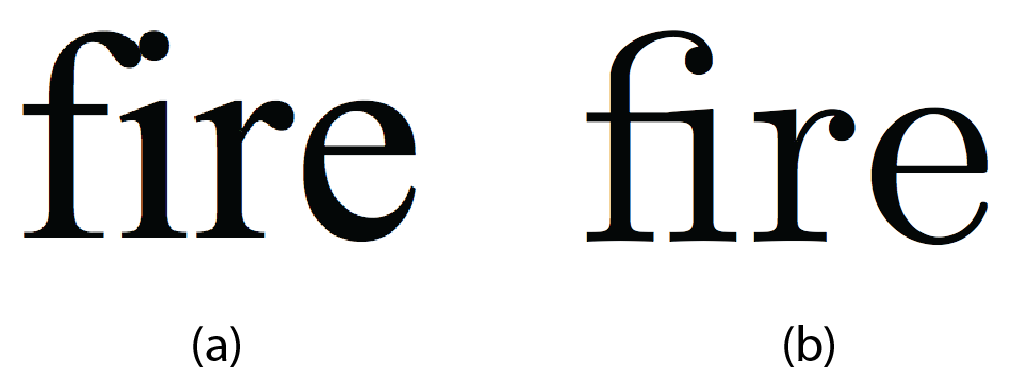
\includegraphics[width=6cm]{images/fireandfire.png}}
\caption{The word `fire' typeset by (a) Microsoft Word 2011 without ligated characters, and (b) by \LaTeX\ showing the ligation of the characters `f' and `i'}\label{figure:twofires}
\end{figure}
%
But that's enough about the typography of the word `fire' for now. Let's put together something more substantial. 

\subsection{Task 2}
\label{sec:task-2}

 Create yourself a new file, called `sections.tex' by copying `fire-and-ice.tex'. In `sections.tex', replace the line of poetry with the text from Figure \ref{figure:bleakhouse} (which contains the first three paragraphs of Dickens' novel, `Bleak House' \citep{dickens1852}).

\begin{figure}[tbp]

\begin{quote}

\itshape
London. Michaelmas term lately over, and the Lord Chancellor sitting
in Lincoln's Inn Hall. Implacable November weather. As much mud in
the streets as if the waters had but newly retired from the face of
the earth, and it would not be wonderful to meet a Megalosaurus,
forty feet long or so, waddling like an elephantine lizard up Holborn
Hill. Smoke lowering down from chimney-pots, making a soft black
drizzle, with flakes of soot in it as big as full-grown
snowflakes--gone into mourning, one might imagine, for the death of
the sun. Dogs, undistinguishable in mire. Horses, scarcely better;
splashed to their very blinkers. Foot passengers, jostling one
another's umbrellas in a general infection of ill temper, and losing
their foot-hold at street-corners, where tens of thousands of other
foot passengers have been slipping and sliding since the day broke
(if this day ever broke), adding new deposits to the crust upon crust
of mud, sticking at those points tenaciously to the pavement, and
accumulating at compound interest.



Fog everywhere. Fog up the river, where it flows among green aits and
meadows; fog down the river, where it rolls defiled among the tiers
of shipping and the waterside pollutions of a great (and dirty) city.
Fog on the Essex marshes, fog on the Kentish heights. Fog creeping
into the cabooses of collier-brigs; fog lying out on the yards and
hovering in the rigging of great ships; fog drooping on the gunwales
of barges and small boats. Fog in the eyes and throats of ancient
Greenwich pensioners, wheezing by the firesides of their wards; fog
in the stem and bowl of the afternoon pipe of the wrathful skipper,
down in his close cabin; fog cruelly pinching the toes and fingers of
his shivering little 'prentice boy on deck. Chance people on the
bridges peeping over the parapets into a nether sky of fog, with fog
all round them, as if they were up in a balloon and hanging in the
misty clouds.

Gas looming through the fog in divers places in the streets, much as
the sun may, from the spongey fields, be seen to loom by husbandman
and ploughboy. Most of the shops lighted two hours before their
time---as the gas seems to know, for it has a haggard and unwilling
look.

\end{quote}

\caption{Some sample text from the opening of the Dickens' novel `Bleak House' \citep{dickens1852}.}\label{figure:bleakhouse}
\end{figure}

Edit the text to make sure that there is a blank line between each of the three paragraphs (it's not enough that each paragraph starts on a new line of its own, there has to be an empty line in between them). That's how paragraphs are distinguished in \LaTeX\ (in fact, it doesn't matter how many blank lines you put as long as there is at least one\ldots for the most part \LaTeX\ ignores spare whitespace). Now type a paragraph of gibberish by randomly hitting keys on the keyboard, and putting spaces in to make `words' in the text file. You should end up with something like the following, but about three times as long (don't cut and paste this from here\ldots it's important that you actually create some unique gibberish yourself!):

\begin{verbatim}
Oisjdf oqweqwe oi soijs hbweo kbsd oijsdf 
oijqwknpiouh iusbdfspb sifuhygwqeb usgweijf 
blimqwoq oieuerwefwiu aokqjw uioshiufds 
qiqks odfubfi psdiweneq.
\end{verbatim}

Be careful at this stage to only include letters (uppercase and lowercase), commas, full-stops and perhaps numbers in your gibberish text: if you use any other symbols, you may upset \LaTeX. 

Next go to the website \href{http://www.lipsum.com/}{http://www.lipsum.com} and follow the instructions to generate yourself three paragraphs of what's called `Lorem Ipsum' text. Copy and paste that text into your \LaTeX\ document too (don't worry about what it means at this stage), again making sure that you have a blank line between the paragraphs.

Re-run \texttt{pdflatex} and look at the resulting `sections.pdf'. Again, at first glance, there's nothing hugely exciting going on here: the text from your .tex file has been assembled into a (probably) two page PDF document. But in fact quite a few things have happened: 

\begin{itemize}
\item The blank lines that separate the paragraphs in your source file are gone, and instead \LaTeX\ has indented the first line of each paragraph. There's nothing profound here about the decision to indent paragraphs rather than (say) to leave a gap between them (so called `block paragraphs'); it's just \LaTeX's default paragraph style, and can be changed easily enough\footnote{Though apparently, there is some evidence in \cite{tinker63} that indented paragraphs increase readability}.
\item There are page numbers at the bottom of each page. This is a very sensible default, allowing you in meetings to ask people to ``turn to page 4'' and so on (it's a bit odd that most wordprocessors don't do this by default too!). But you can easily switch page numbers off, change their style or move them elsewhere if you need to. 
\item The text is `fully justified' so that it's flush on both the left and right hand edges.
\item Certain words that fall at the end of lines have been hyphenated, even if they weren't originally split by hyphens in the source text.
\end{itemize}

These last two points about justification and hyphenation might seem utterly trivial, but getting these factors right turns out to be an important part of making readable documents; readability is not just about which font you choose, but about how the characters and spaces are distributed on each line. It's something that you will have seen happen so often in professionally typeset materials that you'll have taken it for granted, and you may not have spotted that it doesn't happen in quite the same way when you use a wordprocessor. The principle behind justifying text seems easy enough at first glance: you simply have to take any `left over' space that would be at the end of a line, and redistribute it between the words in some way to `space them out' a bit more so that they take up all the available horizontal room. But it turns out to be much harder than it seems, and all the simple ways you might think of for doing this on a per-line basis give results that are visually quite unsatisfactory, with nasty patterns made up of neighbouring whitespace appearing in the layout and ruining everything. The added complication here is that to do the optimum job of shuffling the words round on their lines, you really need the flexibility of being able to hyphenate words to give you extra space on lines that would otherwise be tightly packed with characters. But if you hyphenate words badly, by breaking them in inappropriate places, or do it too often then that makes the text hard to read too. It's all deeply inconvenient and inter-related. The best solution to this aesthetic conundrum so far was developed by \cite{SPE:SPE4380111102} and later improved by Frank Liang during his PhD research \citep{liang}, and it's a technique that tries to optimise the layout of whole paragraphs rather than individual lines. The algorithm takes into account all manner of different things: language-specific character patterns, the number of consecutive lines that end with hyphens, the word `tightness' on each line\ldots any many others. The details don't really matter here, but the really important thing insight is that you get better results by working on a bigger chunk of the document (in this case a paragraph at a time) rather than trying to independently optimise lots of small bits (say, lines) and hoping that the result of joining them all together turns out nicely. This idea of optimising things `globally' versus `locally' is something you'll see many times throughout your Computer Science degree; watch out for it in all the algorithms courses.

This highlights a fundamental difference between the WYSIWYG para\-digm and the way that documents are produced using \LaTeX. As we've seen, small changes down the the level of individual characters can have fairly large knock-on consequences for the optimal layout of a document: changing one letter for another affects the length of a line, which in turn affects the hyphenation options, which then affects the length of a paragraph, which means that the best place for a figure that was on page 99 might now on page 100, but that means that all references to `page 99' now need a bit more room to account for the extra digit which means that the some line lengths have changed which means\ldots well, you get the idea. It's more complicated that it first seems. \LaTeX\ gets to see the \emph{whole of your document at once}, and can therefore make decisions about how best to hyphenate lines,  position figures or whatever else it likes \emph{before} it shows you the results; so it can make solutions that are optimal for the whole document, as well as looking at details such as ligated characters. Wordprocessors can't afford to do this since it would be deeply distracting if every time you typed a character, the whole layout of the document flapped around in front of your eyes. Wordprocessors can only sensibly make little optimisations at a local (probably per-line level). It's not that wordprocessors are rubbish, or that the people that programmed them were lazy: it's a fundamentally different way of working, and knowing the pros and cons of the different approaches will help you pick the right tool for the job. 

You may have noticed that actual text in your document (and in fact, this one) takes up a (perhaps) surprisingly narrow horizontal region of the page. This last `feature' might seem odd at first, but it illustrates another important typographical point that you may never have thought of before: reading long lines of text is hard, because your eyes find it hard to move in a completely straight line as they scan from left to right. So the longer the line of words, the more you have to work to keep your eyes from accidentally drifting up or down onto a neighbouring line (perhaps you've experienced the phenomenon of accidentally re-reading the same line over and over as your eyes get tired). It may never have occurred to you, but most books have relatively short lines of text; and those that use large pages often split text into several columns so that individual lines are kept relatively short. The widely trusted book ``The Elements of Typographic Style'' \citep{bringhurst92} makes the following assertion:

\begin{quote}
\emph{
``Anything from 45 to 75 characters is widely-regarded as a satisfactory length of line for a single-column page set in a serifed text face in a text size. The 66-character line (counting both letters and spaces) is widely regarded as ideal.''}
\end{quote}

\LaTeX\ knows about this issue, so made a sensible default decision for you. 

There's one last unusual thing to note: your paragraph of gibberish text in between the real words from Bleak House and the Lorem Ipsum almost certainly stands out and looks really quite odd (it might even have confused \LaTeX's hyphenation rules enough to have ended up with one or more lines sticking out proud of the right hand margin).  Let your eyes relax so that your vision blurs for a moment: you can still probably spot that the gibberish paragraph looks out of place. It's quite likely that you even found creating the gibberish unexpectedly hard. The interesting thing here is that as humans, we spend so much time reading and writing `proper' natural language that we become attuned to the patterns of letters words and the underlying `rhythm' of our written language that its very hard to artificially reproduce something that looks plausible; the frequency of the letters you chose by randomly hitting keys, and the length and patterns of the words you put in place most likely don't match the natural patterns of real languages, so they just look plain wrong.  Curiously the Lorem Ipsum text that you got from the website probably doesn't look so bad, in spite of it not being made up of real words. But that's not surprising since `Lorem Ipsum' is specifically created to be used as a placeholder for real text when typesetting. While the words are meaningless Latin-like things, their length, and the distribution of characters and word lengths are chosen to mimic patterns in real language.

\subsection{Task 3}
\label{sec:task-3}

Next let's give our document some structure by dividing it up into sections. On the line before Bleak House starts, add the command

\begin{verbatim}
\section{Bleak House}
\end{verbatim}
%
making sure it appears on a line of its own. Then just before your paragraph of gibberish, put similar a similar instruction (again, on its own line), and then create a final section before the Lorem Ipsum. Rerun pdflatex and look at the results. You should see the section headings appear in the appropriate places in the PDF, automatically having been given section numbers. Experiment by adding in a couple of sub-sections towards the end of the document using the  \verb|\subsection| command, which like \verb|\section| command above takes as a parameter some text in contained in wiggly brackets. 

Now, at the top of your document after the \verb|\begin{document}| line and before the command defining the first section, add the following two commands, each on their own line:

\begin{verbatim}
\tableofcontents
\newpage
\end{verbatim}
%
  Re-run pdflatex, and check that the effect is what you'd expect!

\begin{note}
    Need to run latex twice here. Tell them? Tell them why?
\end{note}

\section{Common formatting features}

Before we give you some more exercises to do, here is a brief introduction to some commonly used features of \LaTeX.

\subsection{Enumerated and bulleted lists}

Creating bulleted or numbered lists in \LaTeX\ is straightforward, and is done like this:

\begin{verbatim}
\begin{enumerate}
\item My first item
\item My second item
\item The last thing on my list
\end{enumerate}
\end{verbatim}
%
You must make sure that you both \texttt{begin} and \texttt{end} your list, and that each item is terminated by a newline. Changing `enumerate' to `itemize' gives you a bulleted rather than numbered list (note the American spelling of `itemize').  

\subsection{Bold and italic text}
Text can be typeset in \textbf{bold} font using the \verb|\textbf|, and \textit{italics} using \verb|\textit| as in the example below:

\begin{verbatim}
Some say the \textbf{world} will end in \textit{fire},
\end{verbatim}

\subsection{Cross referencing}

\LaTeX\ allows you to cross-reference almost anything in the document, which includes sections, sub sections and figures. To use the cross-referencing feature you simply insert the command 
\begin{verbatim}
\label{mymarker}
\end{verbatim}
at the point in the document you want to refer to, and then use the command

\begin{verbatim}
\ref{mymarker}
\end{verbatim}
when you want to use the reference. Obviously you replace the text `mymarker' with something more meaningful. An important tip here is to call the marker something that refers to the content of that part of the document, and to avoid the temptation to use numbers (so don't call your marker `section1', instead call it `introduction'; if you reorder your document, it's still likely to be the introduction, but it may no longer be Section 1). For example:

\begin{verbatim}
\section{Reflection on Welcome Week}
\label{welcomeweek}
I spent most of welcome week getting to know my way
around campus. I should have made more effort to join
societies I think; I must remember to get to the
Students' Union and take a look around there.

\subsection{Things I enjoyed}
Everything so far has been wonderful, with the caveat I 
mentioned in Section \ref{welcomeweek}.

\subsection{Things I didn't enjoy}
I've discovered that I don't like soggy chips.
\end{verbatim}

The really useful thing about cross-referencing in \LaTeX\ is that you'll get warnings when you compile your document if cross-references are undefined or used incorrectly. This means you don't have to manually check every reference in your document to make sure its still right.

\begin{note}
  Run twice?
\end{note}

\subsection{Figures and pictures}

Including figures and pictures in your document is easy. You do it like this:

\begin{verbatim}
\begin{figure}
\centerline{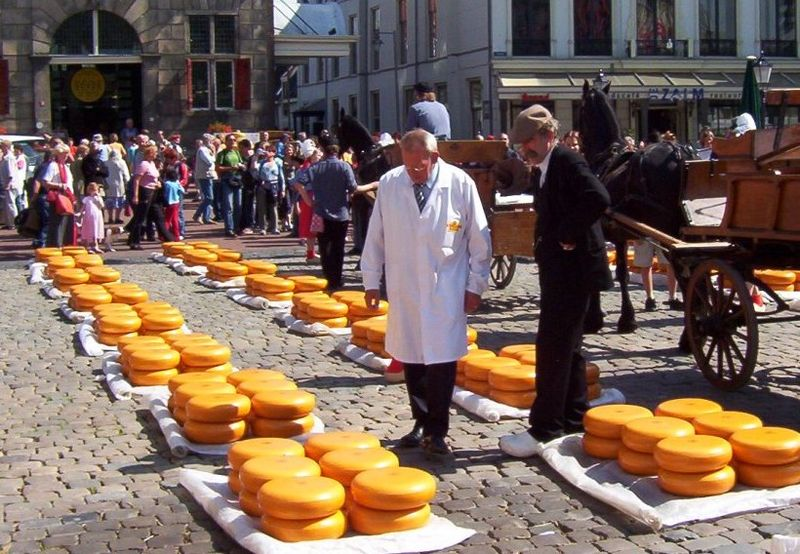
\includegraphics[width=10cm]{images/men-and-cheese.jpg}}
\caption{Some men, possibly Dutch, looking at cheeses.}
\label{figure:menandcheeses}
\end{figure}
\end{verbatim}
which we used to create Figure~\ref{figure:menandcheeses}. You can probably see what's happening. \verb|\includegraphics{}| gets your image, which can be PDF, PNG, JPG, GIF or PostScript. The \verb|\begin...\end| code ``wraps'' up whatever picture you're including, and allows \LaTeX\ to treat it as an unbreakable ``floating'' thing that it will position for you as best it can in the document, while maintaining an overall nice typographical layout. This ``floating'' of figures can sometimes result in the figure ending up in a place you didn't expect, but in most cases \LaTeX\ will make the most sensible choice. It's possible to exercise finer control over figure placement, but that's beyond the scope of this exercise.

\begin{note}
  Need \verb+\includepackage{graphicx}+
\end{note}

\subsection{Typesetting Mathematics}
\label{mathssection}

Earlier we saw this formula:

\[ x = \frac{-b \pm \sqrt{b^2-4ac}}{2a} \]
It looks nice, doesn't it? To tell \LaTeX\ to display this, you have to type a bit of magic, but it's easily-learned magic. To create such a formula in a WYSIWYG editor, there is also magic involved, but it usually involves a lot of mouse-clicking, and remembering special key combinations like 'control-this' and 'alt-that'. In \LaTeX\ it doesn't. You simply type this:
\begin{verbatim}
     \[ x = \frac{-b \pm \sqrt{b^2-4ac}}{2a} \]
\end{verbatim}
You can probably work out how most of this creates the formula, but it won't be obvious that the \verb|\[| and  \verb|\]| characters that enclose the formula mean ``typeset this as a displayed formula, giving it some vertical space from the surrounding text''. If we'd used \verb|\(| and \verb|\)| instead to enclose the formula it would appear in-line, like this: \(  x = \frac{-b \pm \sqrt{b^2-4ac}}{2a} \). It still looks very nice, and observe how it's automatically been resized to fit, and that the lines of text have had their spacing changed a bit. This all looks simple, but the implementation inside \LaTeX\ and \TeX\ is complex. It involves parsing the description of the formula to create a corresponding tree data structure, which is then recursively ``walked'' to work out the horizontal and vertical typographical spacings needed. You'll meet these ideas in \courseunit{COMP11120} and \courseunit{COMP26120} Algorithms and Imperative Programming.

Here's another example, taken from \courseunit{COMP27112} Computer Graphics (it's a `simple' local illumination model incorporating ambient, diffuse and specular reflection by multiple lights):

\[ I = k_a I_a + \sum_{i=1}^M {\frac{{I_p}_i}{d'_i}} [ k_d(\hat{N}\cdot\hat{L_i}) + k_s(\hat{R_i}\cdot\hat{V})^n] \]
%
We write this in \LaTeX\ as follows:

\begin{verbatim}
    \[ I = k_a I_a + \sum_{i=1}^M { \frac{{I_p}_i}{d'_i} }
    [ k_d(\hat{N} \cdot \hat{L_i}) 
    + k_s(\hat{R_i} \cdot \hat{V})^n] \]
\end{verbatim}
%
Try to match the \LaTeX\ commands with the formula displayed above. You'll see lots of curly brackets, and this example illustrates their two uses in \LaTeX. The first is to provide an argument to a command; for example \verb|\hat{N}| means ``apply the \verb|\hat| command to $N$'', which creates \(\hat{N}\), the vector \( N \) with a little hat  on.  

The second use of curly brackets is to group things together to avoid ambiguities. In the example you can see \verb|\sum_{i=1}^M|, which creates a summation sign and its lower and upper limits: \( \sum_{i=1}^{M} \). We wrap the lower bound, \verb|i=1|, in curly brackets to group it into an indivisible unit. If we were to omit the brackets, writing \verb|\sum_i=1^M|, \LaTeX\ would then produce \( \sum_i=1^M \), which is not at all what we want (even \LaTeX\ can't always know what we really want).

One final example. If we tell \LaTeX:

\begin{verbatim}
   \[ T_1 = \left[
    \begin{array}{cccc}
    \cos \theta & -\sin \theta & 0 & \delta \\
    \sin \theta  & \cos \theta & 0 & \epsilon \\
    0 & 0 & 1 & \eta \\
    \alpha & \beta & \gamma & 1
    \end{array}
    \right] \]
\end{verbatim}
%
we'll get a splendid matrix which expresses a particular 3D geometrical transformation (don't worry if you don't recognise this, you'll be introduced to matrix notation in the latter part of \courseunit{COMP11120}: Mathematical Techniques for Computer Science. For now you can just treat it as `some maths'):

\[   T_1 = \left[
    \begin{array}{cccc}
    \cos \theta & -\sin \theta & 0 & \delta \\
    \sin \theta  & \cos \theta & 0 & \epsilon \\
    0 & 0 & 1 & \eta \\
    \alpha & \beta & \gamma & 1
    \end{array}
    \right]
\]
%

In the \LaTeX\ code,  \verb|\left[| means ``big opening square bracket please'';  \verb|{cccc}| means ``an array with 4 columns please, with the items in each column centred"; \verb|&| means ``start a new column''; and \verb|\\| means ``start a new row''. You'll notice that \LaTeX\ knows about  greek letters; it knows about all standard maths symbols too, and also they ways  they're usually used.


\subsubsection{A longer piece of maths}
\label{sec:longer-piece-maths}

  We conclude this section with an example of a longer piece of mathematics, that shows how you might typeset a complete mathematical argument rather than a single formula. The example is Euclid's proof of the fact that $\sqrt{2}$ is irrational. It's an argument that has been covered in COMP11120 and is an example of proof by contradiction. It starts by making the assumption that it is \emph{not the case} that $\sqrt{2}$ is irrational, in other words that we can find integers $p$ and $q$ with $\sqrt{2} = p/q$.

  We can assume, without losing anything, that $p$ and $q$ have \emph{no common factors} (Why?)
  \[
  \begin{array}{lcl}
     \sqrt{2} & = & p/q \\ 
      q\sqrt{2} & = & p\\ 
      2q^2 & = & p^2\\ 
  \end{array}
  \]
  This means that $p^2$ is even, from which we can also deduce that $p$ is even. (Why?)

  This means that $p = 2k$, for some $k$, so \ldots
  \[
  \begin{array}{llcl}
      & 2q^2 & = & (2k)^2\\ 
      \therefore & 2q^2 & = & 4k^2\\ 
      \text{so} & q^2 & = & 2k^2\\
   \end{array}
  \]
  But this means that $q^2$, and hence $q$ is  even. Since $p$ and $q$ are both even we have a contradiction to our initial assumption, so no such $p$ and $q$ exist.

To see how this is done, please look at the source of this document.

\begin{note}
  are we really going to publish the full source, or just bits like this?
\end{note}

  \LaTeX\ really shines at typesetting mathematics, and it would take pages and pages to describe all the features. Have a look at:
\\
\\
\href{http://en.wikibooks.org/wiki/LaTeX/Mathematics}{http://en.wikibooks.org/wiki/LaTeX/Mathematics}
\\
\\
for a flavour. 
 
\section{More exercises}

\begin{note}
  Insert versions some of existing lab exercises here.
\end{note}

\subsection{Task 1: A reflection on your studies}
Your first \LaTeX\ document will be a very brief reflection on your studies so far.

You should work in \verb+$HOME/COMP10120/ex3+. Write a hand-crafted \LaTeX\ document called 
\fname{courses-reflection.tex} (exact name please, otherwise submit will not work). It will have the following structure.

\begin{enumerate}
\item 
Appropriate title including author and date.
\item Table of contents.
\item A brief paragraph saying what the document is about.
\item  A section, appropriately titled, for one of your courses, containing:
  \begin{itemize}
  \item  a brief paragraph saying what the course is about. This will contain a citation referring to the URL of the course syllabus page.
 \item A sub-section, appropriately titled, containing an enumeration of the three things you like the most about the course.
\item A sub-section, appropriately titled, containing an enumeration of the three things you like the least about the course.

  \end{itemize}
 A repeat of item 4 for each other course you are studying. These sections should appear in alphabetical order by course code (e.g. COMP10120).
\end{enumerate} 
After completing and successfully `compiling' and viewing your document, you should spell-check it as follows.

\begin{ttoutenv}
ispell courses-reflection.tex   
\end{ttoutenv}

Once you are completely satisfied with it, produce a hard copy ready for marking.


\subsection{Task 2: Arguments about software patents}
\label{sec:task-2:-arguments}

\begin{note}
  This won't work and needs replacing
\end{note}

In this task you will create three documents which have two shared parts in common. All together you will create five files as follows (please be exact with the filenames).

pros-and-cons.tex This will be a document that contains the pros and cons of software patents. It will contain a paragraph explaining what the document is about, a section listing the pros, another section listing the cons and finally a section concluding the balanced argument.
for.tex This will be a document that contains only the pros of software patents. It will contain a paragraph explaining what the document is about, a section listing the pros and finally a section concluding the argument for software patents.
against.tex This will be a document that contains only the cons of software patents. It will contain a paragraph explaining what the document is about, a section listing the cons and finally a section concluding the argument against software patents.
pros.tex This will be a piece of \LaTeX\ (not a full document) that will be included in the first and second document.
cons.tex This will be a piece of \LaTeX\ (not a full document) that will be included in the first and third document.
Just to be clear, you will not cut and paste the pros and cons lists into the two documents they each finally appear in. Instead you will arrange for the file containing each list to be input by the two documents. The idea here is that if you think of more pros or cons, or wish to change the wording of any, you can edit the corresponding single file, and the changes will appear in both documents that use it. You will need to find out how to make a \LaTeX\ source file input another one.

\subsection{Task 3: A neat directory listing (optional)}
The fact that \LaTeX\ source files are just text makes it easy to have them generated by a program. You are going to exploit this and use \LaTeX\ to produce a neat document containing a listing of the files in any directory.

Find out about \LaTeX\ tables (the tabular environment).
Make a \LaTeX\ document by hand that uses a table to neatly show the information about the files in some (small) directory (as produced by ls -l).
Write a shell script, called neat-ls, that takes an argument which is the path name of a directory, and produces a \LaTeX\ document containing the above table for the given directory. The script could also process the \LaTeX\ and display the resulting dvi file.
Finally, find out about the longtable package and change your script to use that instead.

\subsection{Task 4: A cleaning rota (optional)}
Now you will write a shell script, called rota, that generates a house cleaning rota. (Very handy for next year ...). This is a table with columns such as Kitchen, Bathroom and Lounge. The rows will be weeks in the year, labelled with a date (e.g. always a Sunday). The idea is that house mates can write their initials in the boxes, promising to clean the corresponding room in that particular week. Start by making a sample table by hand.

Your script should take a single argument which is the date of the first row, e.g. Sun 02 Sep 07 - Sat 08 Sep 07. The result will be a document that contains as many rows as fit on a single page (find out by experimenting).

The dates of each row should be generated from the first. See the manual page for date to figure out how you can generate a date that is a number of weeks and days later than an existing one.


\subsection{Task 4}
\label{sec:task-4}

\begin{note}
  Tasks need numbering properly!
\end{note}

 Now for an exercise that involves some mathematics. Please create a file \texttt{f-w.tex} which typesets the following piece of text and mathematics.
\begin{center}
  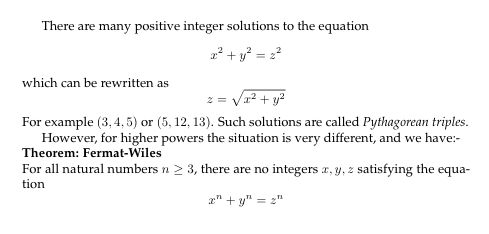
\includegraphics[width=.95\textwidth]{images/f-w}
\end{center}


\section{Next steps}

\LaTeX\ is a very powerful tool, and it does take a little getting used to. But it's not as scary as it might initially seem, and you should find that it doesn't take long to learn the common commands and techniques to make your documents well-structured and readable. As you become more comfortable with the basics and understand the principles of typesetting, finding out how to do more complex and sophisticated things is easy---there are hundreds of tutorials on the web. 

Don't get carried away though, and use the features judiciously: just because you've found a cool new command doesn't mean that you should use it just to show off your \LaTeX\ skills: content and structure always trumps typographic twiddlings\footnote{For example, footnotes like this are, for some reason, a really tempting feature to use in \LaTeX, and in this document we have abused them mercilessly to illustrate a point. Footnotes were originally a means for mechanical typesetters to insert comments, corrections or additions to existing documents without having to adjust the layout of a whole page, and of course in digital typography this is no longer necessary. They can justifiably be used for citations (though it's not common do to do these days) and URLs if you don't want these intruding into the body of your text. And in some very very rare cases, they can be used as an `aside' to the main flow of the text (which is what has been done in this document). But this should be used sparingly\ldots. If something is important to say, put it in the main body of your text. If it's not, then perhaps you should think about leaving it out completely, or find some other way of including it. Asking the reader to look down at the bottom of a page to find out whether something is important or not is irritating, and as you've probably found out already, often means you lose track of your reading position. They also give the impression that the author isn't clear about whether something is important or not, which is never good. And long footnotes like this one---while \LaTeX\ will typeset them perfectly well---are just plain silly. Best avoid.}.

\section{Acknowledgements}

This document is based on an original lab exercise created and written by Dr. John Latham. Some pieces of the original text remain and are included with his permission.  The images in Figure \ref{figure:knuthlamport} are from Wikimedia Commons, via the wikipedia articles on Knuth and Lamport, and are in the public domain. Figure \ref{figure:wordperfect} is from Wikimedia Commons, via the wikipedia article on \href{http://en.wikipedia.org/wiki/WordPerfect}{WordPerfect}, and is in the public domain. Likewise, for Figure \ref{figure:menandcheeses} from the Wikipedia article on \href{http://en.wikipedia.org/wiki/Cheese}{cheese}. Figure \ref{figure:broccoli}, also via Wikimedia Commons, is reproduced with the permission of its creator \href{http://commons.wikimedia.org/wiki/User:Fir0002}{\emph{Fir0002/Flagstaffotos}} under the terms of the \href{http://commons.wikimedia.org/wiki/Commons:GNU_Free_Documentation_License_1.2}{GNU Free Documentation License}. Figure \ref{figure:movabletype} is a combination of images by Daniel Ullrich and Willi Heidelbach, both from wikipedia and both released under the GNU Free Documentation License.

\printbibliography[heading=subbibliography]
\end{refsection}
\endinput

\section{License}

The text of this exercise is licensed under the terms of the \href{http://creativecommons.org/licenses/by/3.0/}{Creative Commons Attribution 2.0 Generic (CC BY 3.0) License}. 

\bibliographystyle{natbib}
\bibliography{latex-exercise}

\appendix

\section{Fire And Ice}
\label{appendix:fireandice}

\begin{quote}
Fire and Ice, \emph{by Robert Frost.}\\

\begin{verse}
Some say the world will end in fire,\\
Some say in ice.\\
From what I've tasted of desire\\
I hold with those who favor fire.\\
But if it had to perish twice,\\
I think I know enough of hate\\
To say that for destruction ice\\
Is also great\\
And would suffice.\\
\end{verse}
\end{quote}

\section{Search Terms}
\label{appendix:searchterms}

dots per inch  / resolution
contrast
LED / LCD / CRT / e-ink
emissive versus reflective
anti aliasing
reading in light / dark environments
annotating / doodling
viewing angles
brightness
levels of colour

use google / google scholar / ACM digital library



Kindle / iPad / eInk / retina display


\end{document} 

Any text, like this, that is after the end of the document is ignored. This can be a
handy place to keep general comments and/or old fragments of the document
which you want to keep.
